\documentclass{abntex2}
\usepackage[utf8]{inputenc}
\usepackage{graphicx}
\usepackage{multirow}
\usepackage[num]{abntex2cite}




\titulo{Experimento 7: Amplificadores operacionais – Resposta em frequência}
\autor{Lucas Rezende de Macedo - 14/0026363\\Jônatas Ribeiro Senna Pires - 14/0090983}
\data{20 de Junho de 2018}
\local{Brasília, Distrito Federal}
\newcommand{\parallelsum}{\mathbin{\!/\mkern-5mu/\!}}

\begin{document}

\imprimircapa
\imprimirfolhaderosto

\tableofcontents
\clearpage
\listoffigures
\listoftables
\clearpage


\chapter{Experiências}

 O objetivo do presente experimento consiste na verificação das características peculiares presentes na resposta
 de amplificadores operacionais reais conforme a variação da frequência.

\section{Experiência}
\subsection{Experiência 1}

Foi montado o circuito de acordo com a figura \ref{fig:circuito}, obtendo, assim, a montagem da figura \ref{fig:montagem1}.
\begin{figure}[h]
  \centering
  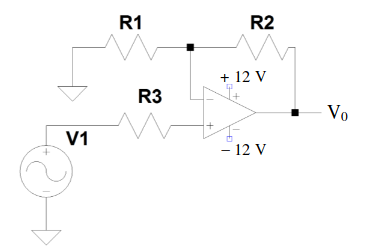
\includegraphics[scale = 0.5]{circuito.png}
  \caption{Circuito amplificador não-inversor com compensação para efeito da corrente de polarização.}
  \label{fig:circuito}
\end{figure}

Para este experimento, esta montagem foram utilizados os seguintes valores (medidos):
\begin{itemize}
  \item $R_1 = 983\Omega$
  \item $R_2 = 9,826k\Omega$
  \item $R_3 = 990\Omega$
\end{itemize}

\subsubsection{Parte 1 - Montagem}

O circuito da figura \ref{fig:circuito} foi montado, obtendo-se a montagem da figura \ref{fig:montagem1}.

\begin{figure}[h]
  \centering
  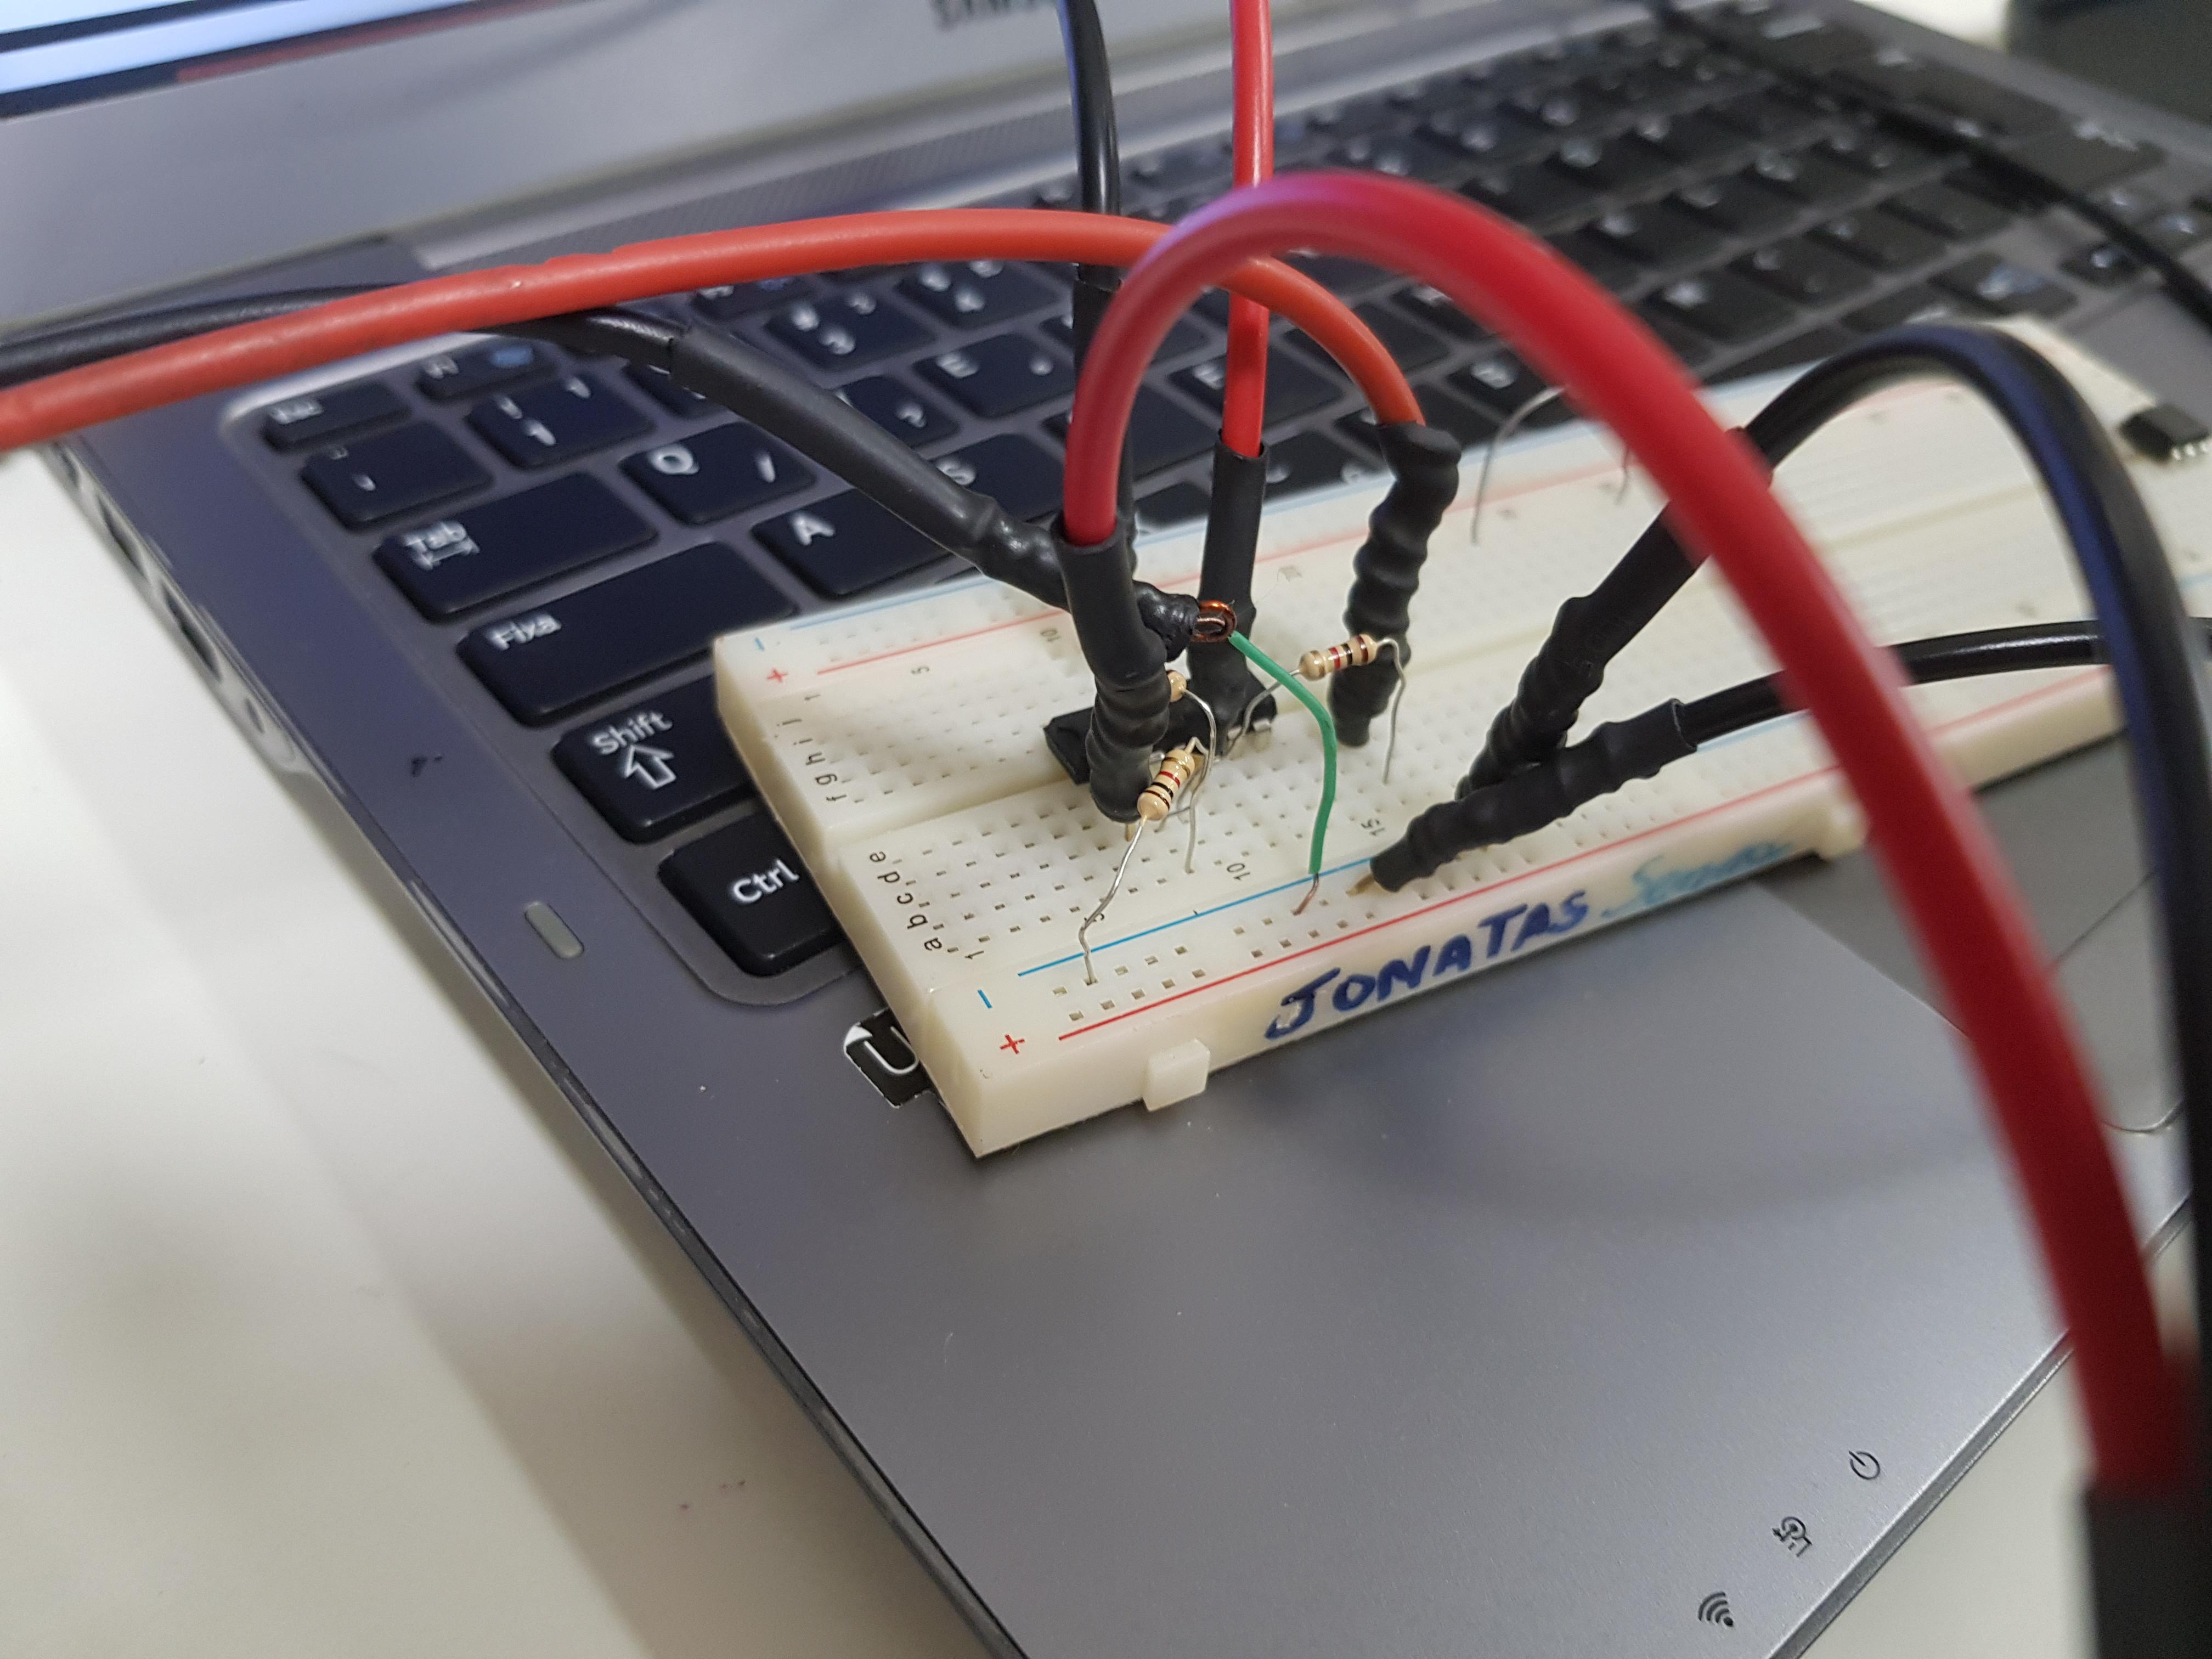
\includegraphics[width = 0.7\textwidth]{montagem1.jpg}
  \caption{Montagem do circuito da figura \ref{fig:circuito}.}
  \label{fig:montagem1}
\end{figure}
Para esta montagem foi escolhido $R_3 = 990\Omega$ de acordo com a seguinte fórmula: \\\\$R_3 = R_1 \parallelsum R_2$

\subsubsection{Parte 2}

Foi ajustada a tensão de entrada para que fosse obtido 1,04 Vpp, ou seja, 0,5 V de amplitude. Ao final do ajuste, $v_i_n = 92 mVpp$ foi o valor que atingiu $V_o_u_t$ desejado, conforme a figura \ref{fig:montagem1}.
\begin{figure}[h]
  \centering
  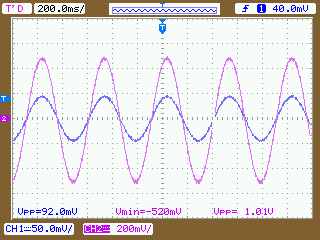
\includegraphics[width = 0.7\textwidth]{NewFile13.png}
  \caption{Gráfico de entrada e saída para o circuito.}
  \label{fig:montagem1}
\end{figure}
\subsubsection{Parte 3}

  Após o ajuste realizado na fase anterior, a frequência foi variada em valores entre 2Hz e 5MHz, obtendo-se os valores contidos na tabela \ref{tab:exp1} a seguir.

  \begin{table}[h!]
  \centering
  \begin{tabular}[width = 0.8\textwidth]{|l|l|l|l|}
    \hline
    Frequência (Hz) & Amplitude $V_I$ (V) & Amplitude $V_O$ (V) & Defasagem entre $V_I$ e $V_O$ ($^{\circ}$) \\
    \hline
    2  & 94m & 1.02 &  2 \\
    \hline
    10   & 94m & 1.02 &  7 \\
    \hline
    30   & 94m & 1.00 &  8 \\
    \hline
    100  & 92m & 1.00 &  5 \\
    \hline
    500  & 92m & 1.00 &  5 \\
    \hline
    1k   & 94m & 1.01 &  7 \\
    \hline
    5k   & 92m & 1.00 &  7 \\
    \hline
    10k  & 92m & 1.00 &  10 \\
    \hline
    30k  & 94m & 992m &  17 \\
    \hline
    50k  & 94m & 944m &  28 \\
    \hline
    100k & 92m & 800m &  50 \\
    \hline
    120k & 94m & 728m &  53 \\
    \hline
    200k & 94m & 528m &  79 \\
    \hline
    500k & 92m & 232m &  115 \\
    \hline
    1M   & 94m & 112m &  144 \\
    \hline
    3M   & 92m & 32m &   - \\
    \hline
    5M   & 88m & 16m &   - \\
    \hline
  \end{tabular}
  \caption{Amplitude e defasagem das tensões $V_I$ e $V_O$ com a variação da frequencia de entrada. Os valores ausentes de defasagem não foram possíveis de ser medidos pelo osciloscópio}
  \label{tab:exp1}
  \end{table}

\subsubsection{Parte 4}
  Para a determinação de frequência de corte, foi verifcado o valor de $V_o$ até que fosse obtido um valor aproximadamente igual a 0,7 vezes o valor de saída original.

\subsubsection{Parte 5}
A diferença de fase na frequência de corte é 53$^\circ$.

%\clearpage

\subsection{Experiência 2}

Foi montado o circuito de acordo com a figura \ref{fig:circuito} com $R1 = 1k\Omega$ e $R2 = 100k\Omega$, obtendo, assim, a montagem da figura \ref{fig:montagem2}.

Dado que $R3 = R1 \parallelsum R2 \approx 990 \Omega$ para minimizar a tensão de offset, foram utilizados os seguintes valores de R (medidos):

\begin{itemize}
  \item $R_1 = 983\Omega$
  \item $R_2 = 100,1k\Omega$
  \item $R_3 = 990\Omega$
\end{itemize}

\subsubsection{Parte 1 - Montagem}

O circuito da figura \ref{fig:circuito} foi montado, obtendo-se a montagem da figura \ref{fig:montagem2}.

\begin{figure}[h]
  \centering
  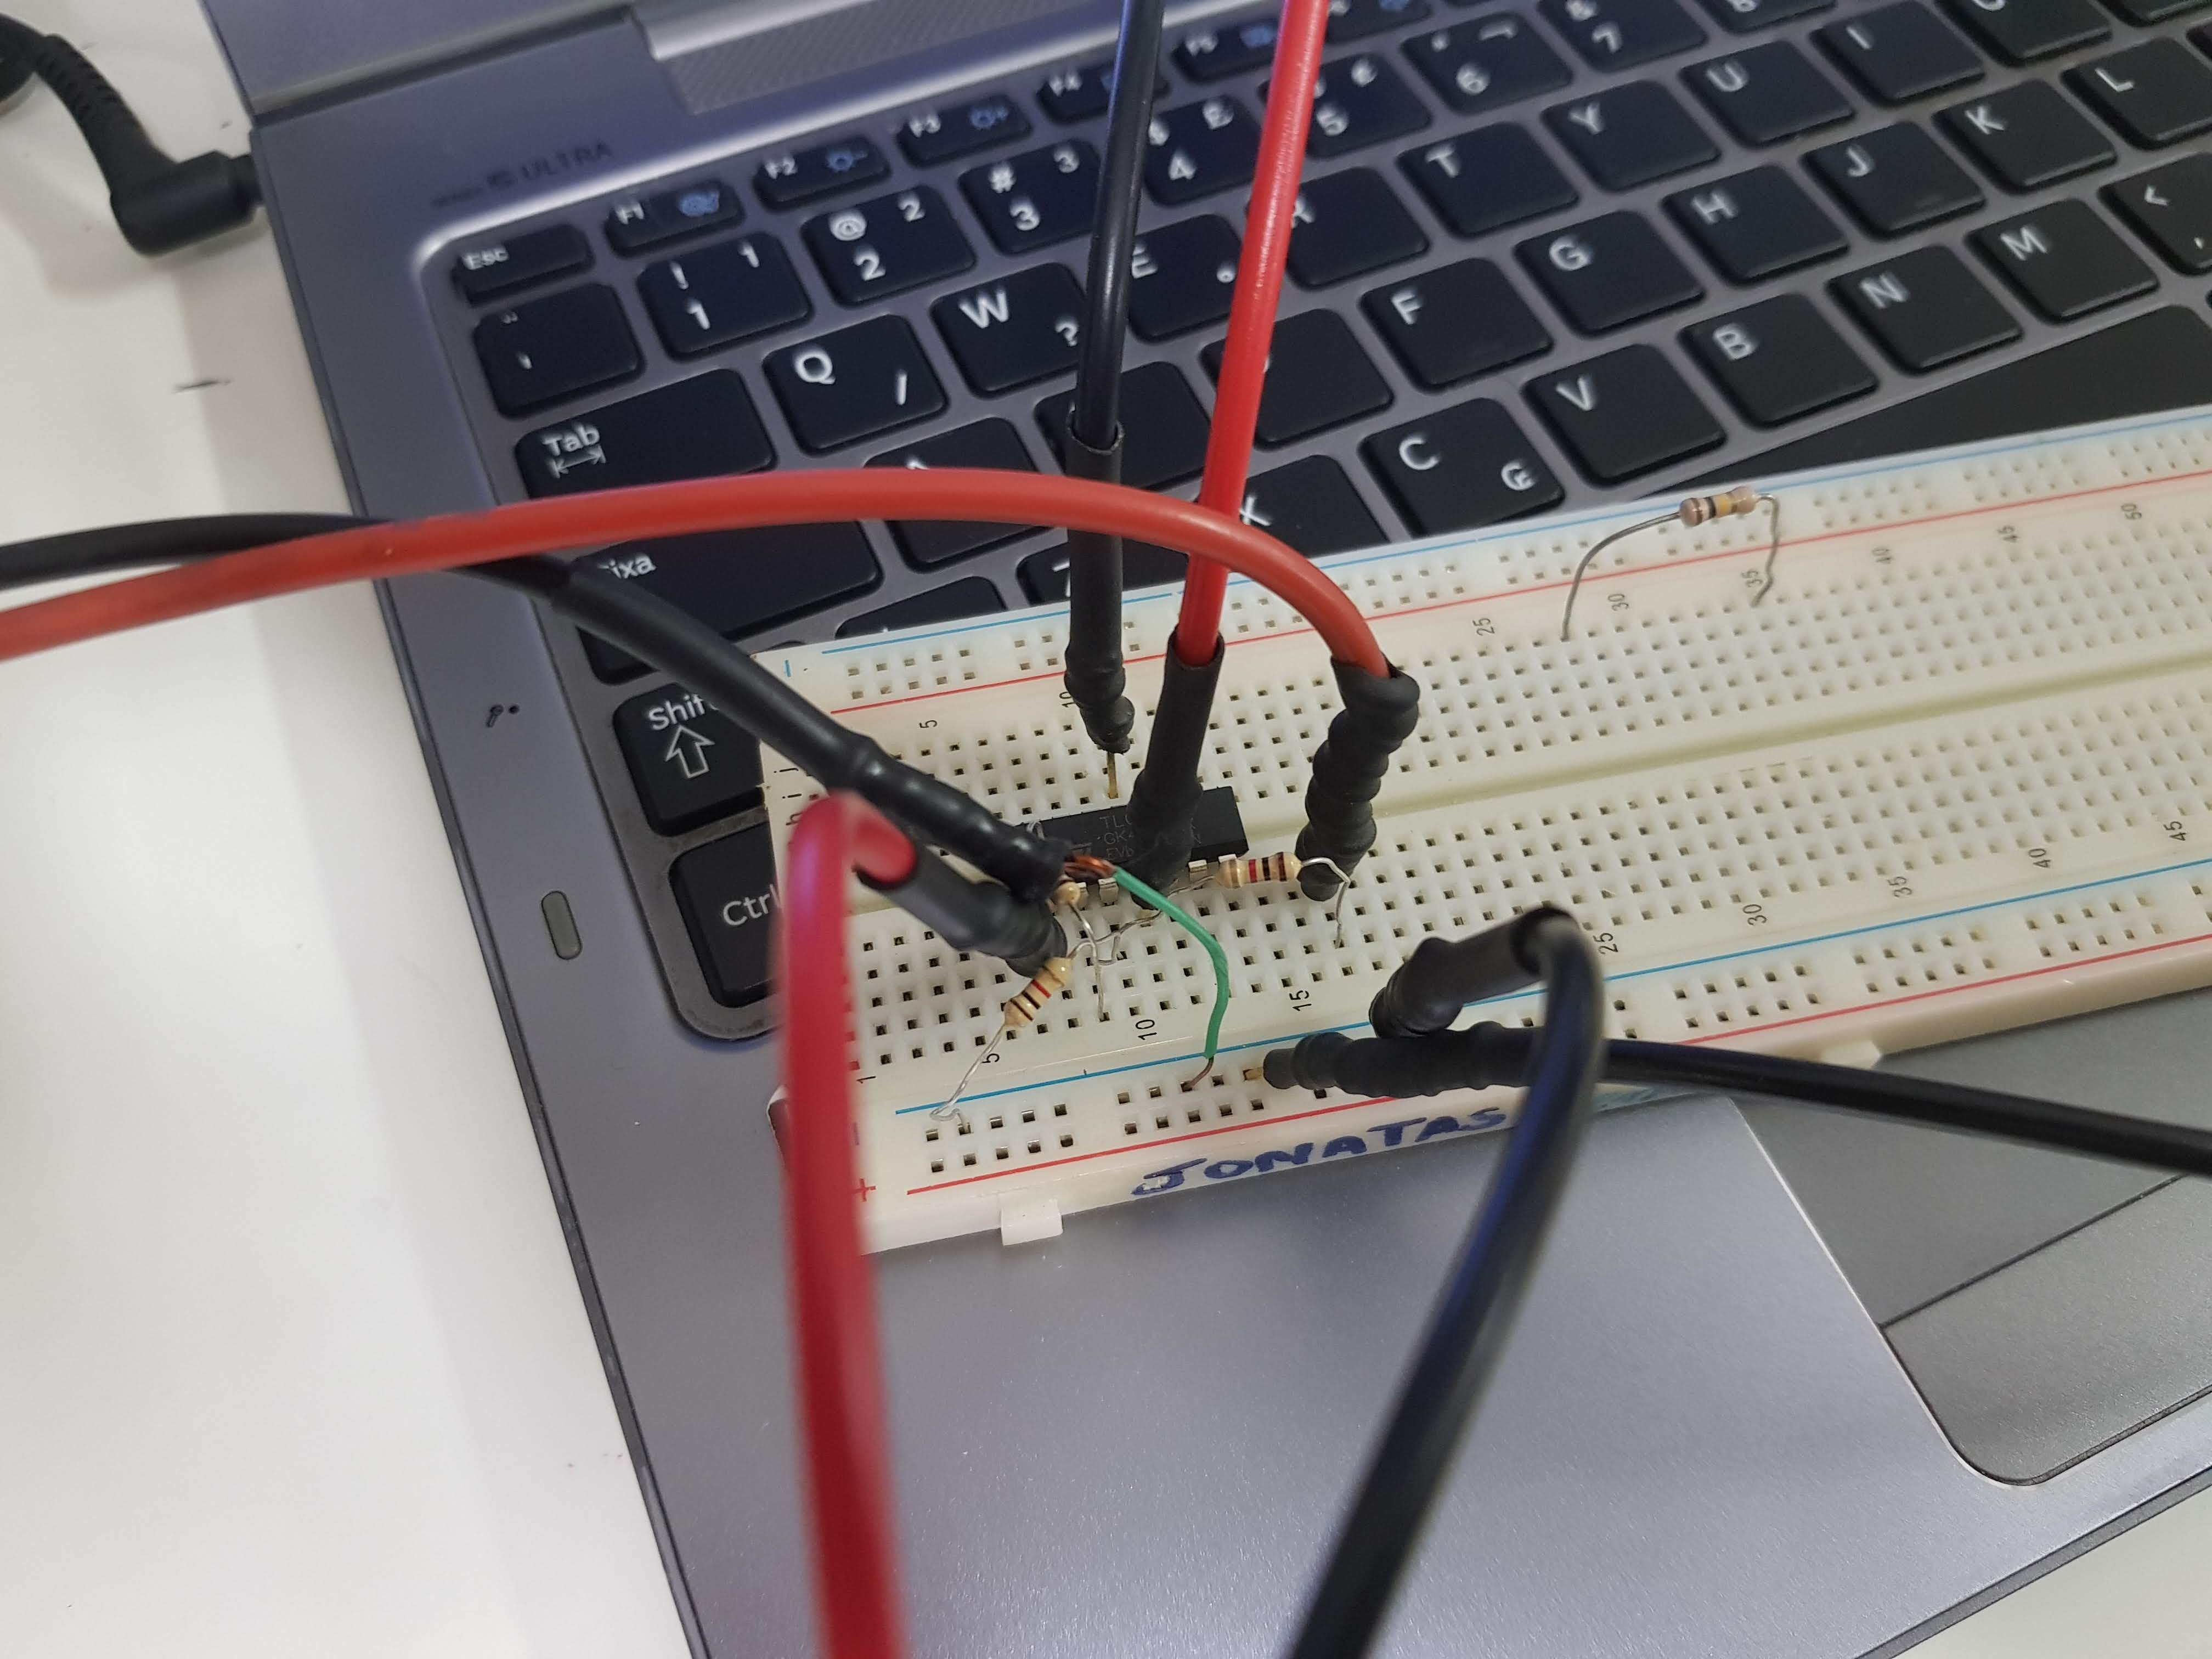
\includegraphics[width = 0.7\textwidth]{montagem2.jpg}
  \caption{Montagem do circuito da figura \ref{fig:circuito}.}
  \label{fig:montagem2}
\end{figure}

\subsubsection{Parte 2}

Para a montagem da figura \ref{fig:montagem2} foi encontrada a frequência de corte de 15 kHz como pode ser observado na tabela \ref{tab:exp2}.

\begin{table}[h!]
  \centering
  \begin{tabular}[width = 0.8\textwidth]{|l|l|l|l|}
    \hline
    Frequência (Hz) & Amplitude $V_I$ (V) & Amplitude $V_O$ (V) & Defasagem entre $V_I$ e $V_O$ ($^{\circ}$) \\
    \hline
    2 & 26m & 2.04 & 7 \\
    \hline
    10 &  23m & 2.00 & 8 \\
    \hline
    30 &  24m & 2.04 & 10 \\
    \hline
    100 & 26m & 2.20 & 14 \\
    \hline
    500 & 24m & 2.08 & 15 \\
    \hline
    1k &  24m & 2.08 & 15 \\
    \hline
    5k &  24m & 1.96 & 30 \\
    \hline
    10k & 24m & 1.68 & 46 \\
    \hline
    15k & 24m & 1.40 & 55 \\
    \hline
    20k & 24m & 1.20 & 60 \\
    \hline
    30k & 24m & 880m & 70 \\
    \hline
    50k & 24m & 560m & 88 \\
    \hline
    100k & 24m & 320m & - \\
    \hline
    500k & 24m & 80m &  - \\
    \hline
    1M &  24m & 40m  & - \\
    \hline
    3M &  24m & 16m  & - \\
    \hline
    5M &  21m & 8m  &  - \\
    \hline
  \end{tabular}
  \caption{Amplitude e defasagem das tensões $V_I$ e $V_O$ com a variação da frequencia de entrada. Os valores ausentes de defasagem não foram possíveis de ser medidos pelo osciloscópio}
  \label{tab:exp2}
\end{table}

\subsubsection{Parte 3}

Pode-se observar que a frequência de corte do amplificador é significativamente menor que a frequência de corte da experiência anterior, isso é esperado porque o ganho do circuito aumentou, o que acarreta na diminuição da frequência de corte.

\subsubsection{Parte 4}

Dado que o ganho teórico para esse circuito é

\[G = 1+\frac{R2}{R1} = 100\]

Para os valores nominais dos resistores $R1$ e $R2$.

Como o valor de \emph{gain-bandwidth product} é igual a 3 MHz para o AmpOp utilizado, tem-se que o valor da frequência de corte em que o $G_{corte} \approx 0.7 G = 70$

\[G_{corte}f_{corte} = 3MHz\]
\[f_{corte} = \frac{3MHz}{G_{corte}} \approx 42,85kHz\]

Observa-se uma diferença consideravel entre o valor teórico de ganho ($42,85 kHz$) e o valor medido ($15 kHz$). Isso se deve ao ganho do AmpOp não ser infinito e apresentar um erro de ganho que não foi levado em consideração no cálculo do valor teórico entre outras não linearidades dos AmpOps.


\chapter{Discussão}

\section{Discussão dos resultados}

Foi possível observar no experimento os fenômenos resultantes da resposta em freqência dos amplificadores operacionais.

Apesar da diferença entre os valores teóricos esperados e os valores medidos ao longo do experimento, o comportamento esperado, dadas as mudanças na freqência de entrada se mantiveram dentro do comportamento esperado pela teoria dos amplificadores operacionais.

\clearpage

\section*{Referências}

[1] SEDRA, Adel S.; SMITH, Kenneth Carless. Microelectronic circuits. New York: Oxford University Press, 1998.

[2] RAZAVI, Behzad; BEHZAD, Razavi. RF microelectronics. New Jersey: Prentice Hall, 1998.

\end{document}
